%% LyX 2.4.3 created this file.  For more info, see https://www.lyx.org/.
%% Do not edit unless you really know what you are doing.
\documentclass[spanish]{article}
\renewcommand{\familydefault}{\sfdefault}
\usepackage[T1]{fontenc}
\usepackage[utf8]{inputenc}
\usepackage{float}
\usepackage{units}
\usepackage{graphicx}
\usepackage{esint}
\usepackage{babel}
\addto\shorthandsspanish{\spanishdeactivate{~<>}}
\deactivatequoting

\begin{document}
\title{Actividad 3 Electromagnetismo I}
\author{Jesús María Mora Mur}
\date{\today}
\maketitle

\section{Densidad de corriente superficial}

Para describir la densidad de corriente superficial, $\vec{K}$, partimos
de la expresión siguiente:

\[
\vec{K}=nI
\]

donde $n$ es el número de vueltas por unidad de longitud. Así, sabemos
que $K=\frac{N\cdot I}{L}$.

Por otro lado, dicha densidad seguirá la dirección del eje axial y
el sentido de la corriente. Por ende:

\[
\vec{K}=\frac{N\cdot I}{L}\hat{z}
\]


\section{Cálculo del campo magnético y caso límite.}

Partimos de la \emph{Ley de Biot-Savart} en su forma diferencial:

\[
d\vec{B}=\frac{\mu_{0}}{4\pi}\cdot\frac{I\cdot d\vec{l}\times\hat{r}}{r^{2}}
\]

Considerando que el elemento de longitud se circunscribe al eje z:

\[
d\vec{l}=dz^{\prime}\hat{z}
\]

Por otro lado, la distancia desde el elemento hasta un punto $z$
del eje axial será:

\[
r=\sqrt{\left(z-z^{\prime}\right)^{2}+a^{2}}
\]

El vector $\vec{r}$ en cilíndricas vendrá dado por una componente
radial y una axial:

\[
\vec{r}=(z-z^{\prime})\hat{z}+a\hat{r_{\phi}}
\]

El producto vectorial tendrá un resultado de:

\[
d\vec{l}\times\hat{r}=dz^{\prime}\frac{a}{\sqrt{(z-z^{\prime})^{2}+a^{2}}}\hat{r_{\phi}}
\]

Sustituyendo en la \emph{Ley de Biot-Savart}:

\[
d\vec{B}=\frac{\mu_{0}}{4\pi}\cdot\frac{I\cdot dz^{\prime}\frac{a}{\sqrt{(z-z^{\prime})^{2}+a^{2}}}\hat{r_{\phi}}}{(z-z^{\prime})^{2}+a^{2}}
\]

Por simetría la componente radial se cancelará. La integral queda
reducida:

\[
\vec{B}(z)=\frac{\mu_{0}Ia}{4\pi}\int_{-\nicefrac{L}{2}}^{\nicefrac{L}{2}}\frac{dz^{\prime}}{(z-z^{\prime})^{2}+a^{2}}=\frac{\mu_{0}NI}{2L}\left(\frac{z+\frac{L}{2}}{\sqrt{\left(z+\frac{L}{2}\right)^{2}+a^{2}}}-\frac{z-\frac{L}{2}}{\sqrt{\left(z-\frac{L}{2}\right)^{2}+a^{2}}}\right)
\]

Si $a\rightarrow0$, entonces $\vec{B}(z)\rightarrow\vec{0}$ fuera
del solenoide.

\section{Gráficas y deducción de conclusiones.}

Podemos comprobar como en el medio interior del solenoide hay campo.
Cuanto más aumentamos la longitud con respecto al radio, más uniforme
es el campo magnético.

\begin{figure}[H]
\centering
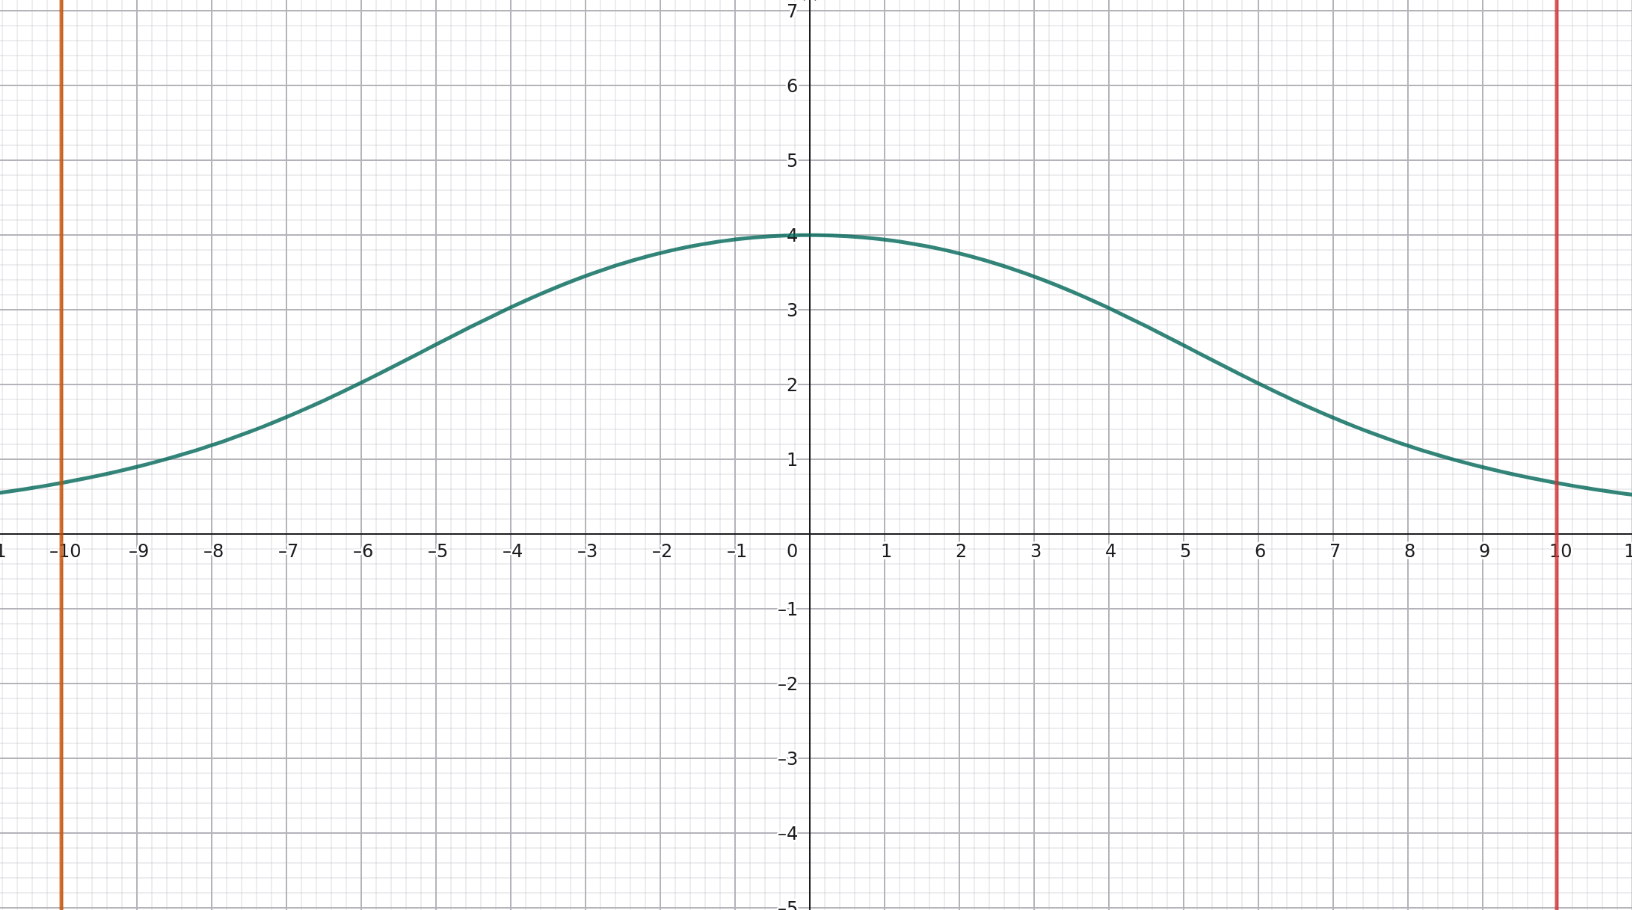
\includegraphics[scale=0.25]{img/grande}

\caption{Apertura grande, $2a=L$}

\end{figure}
\begin{figure}[H]
\centering
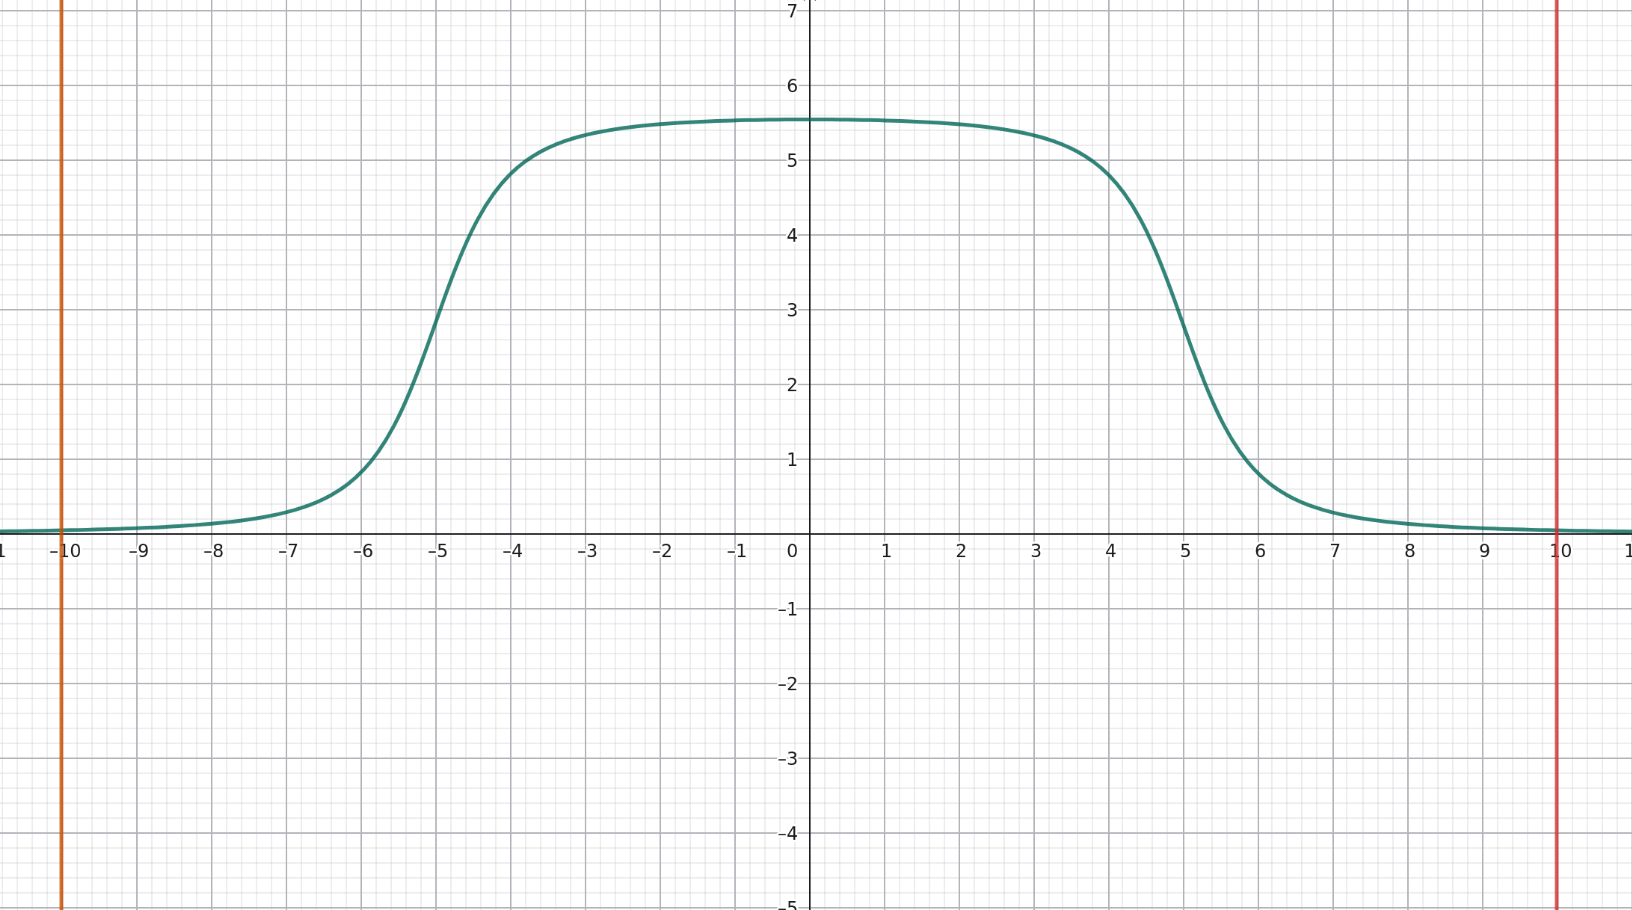
\includegraphics[scale=0.25]{img/mediana}\caption{Apertura mediana, $2a=\nicefrac{L}{5}$}

\end{figure}
\begin{figure}[H]
\centering
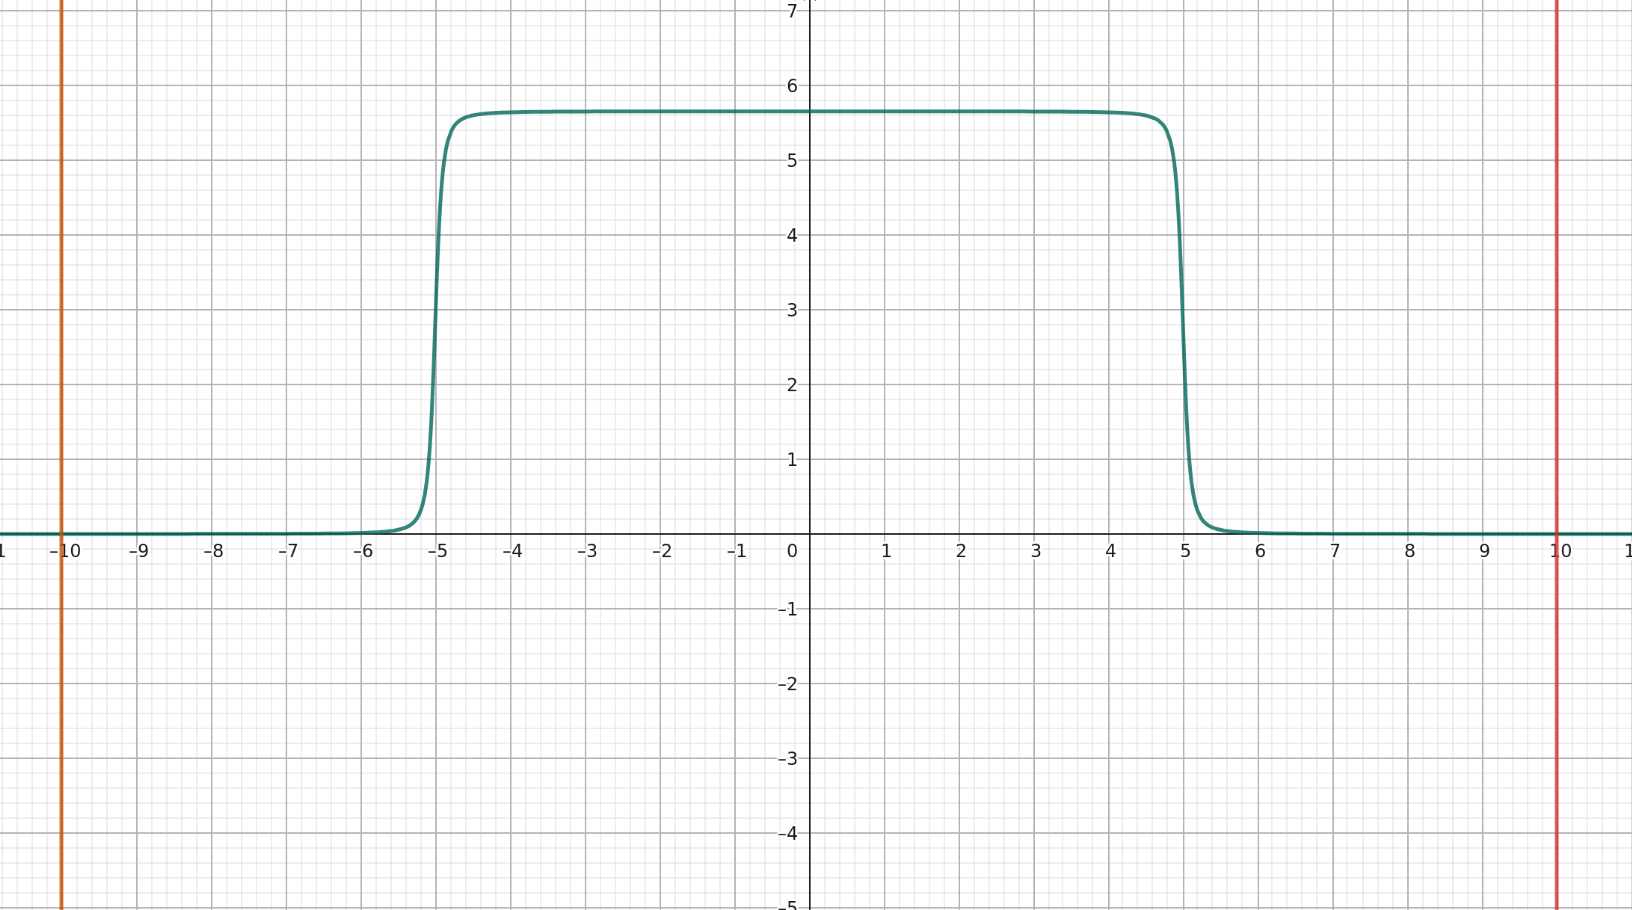
\includegraphics[scale=0.25]{img/pequena}\caption{Apertura pequeña, $2a=\nicefrac{L}{50}$}

\end{figure}

\end{document}
